% !TEX root = ../my-thesis.tex
%
\chapter{Further Analysis using R-Shiny}\label{ch:shiny}
R-Shiny is a framework that enables the creation of web applications and dashboards to visualize data interactively, to make statistics accessible to people without programming skills or a mathematical background, or to enable further analysis on research questions, to name just a few use cases. Dashboards have also been used by governments during the pandemic to effectively communicate infection data related to Covid-19. One example is the Robert Koch Institute's Covid-19 Dashboard, which displays daily infection figures for each municipality in Germany that can be grouped by age group and gender. It displays key figures such as the 7-day incidence and contains a choropleth map, among other features. The dashboard can be accessed at
\begin{center}
    \href{https://experience.arcgis.com/experience/478220a4c454480e823b17327b2bf1d4}{https://experience.arcgis.com/experience/478220a4c454480e823b17327b2bf1d4}
\end{center}
A similar dashboard is available for Norway and specifically for the municipality of Oslo:
\begin{center}
    \href{https://experience.arcgis.com/experience/742a281a0fa74ab79147a76e6b52833b}{https://experience.arcgis.com/experience/742a281a0fa74ab79147a76e6b52833b}
\end{center}
As part of this thesis, a dashboard was developed using the R-Shiny framework, with the intention to give the reader a bit more insight into the data. The dashboard comes with four main features:
\begin{itemize}
    \item[1.] The Data Explorer
    \item[2.] The SIR for Norway and Germany
    \item[3.] Spatial Modelling
    \item[4.] Temporal Modelling
\end{itemize}
\clearpage
\subsubsection*{The Data Explorer}
The main idea behind the data explorer is to display the data used to create all the models fitted in this work. The data can be visualized for Norway, Germany or Europe. Each tab contains a map and several drop-down menus where the user has different choices. For Norway and Germany, in addition to the variable to be displayed on the map, there is also the option to choose between three map types, hexagon maps, heat maps and choropleth maps. Hexagon maps can be seen as a mixture of a heat map and a histogram. Each bar represents the number of times a feature is present within a certain radius. The higher a bar is, the more often the feature is present. Figure~\ref{fig:map_1} shows the number of bakeries within a radius of 2.5 km. It is clear that most bakeries are found in Berlin and Munich.
\begin{figure}[H]
    \centering
    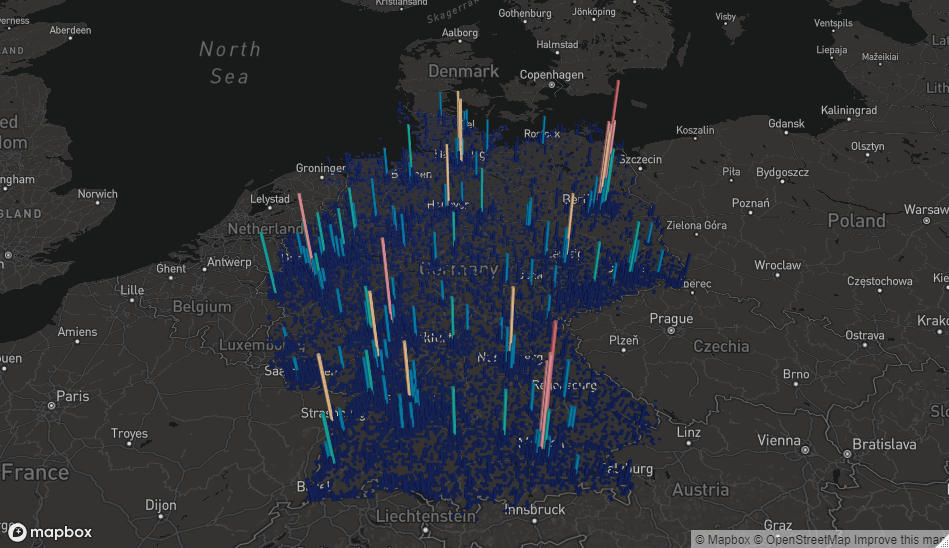
\includegraphics[width = \textwidth]{bakeries_germany_hex.png}
    \caption{A hexagon map of all bakeries in Germany.}
    \label{fig:map_1}
\end{figure}
\clearpage
The same information can also be conveyed using a heat map, as shown in Figure~\ref{fig:map_2}. 
\begin{figure}[H]
    \centering
    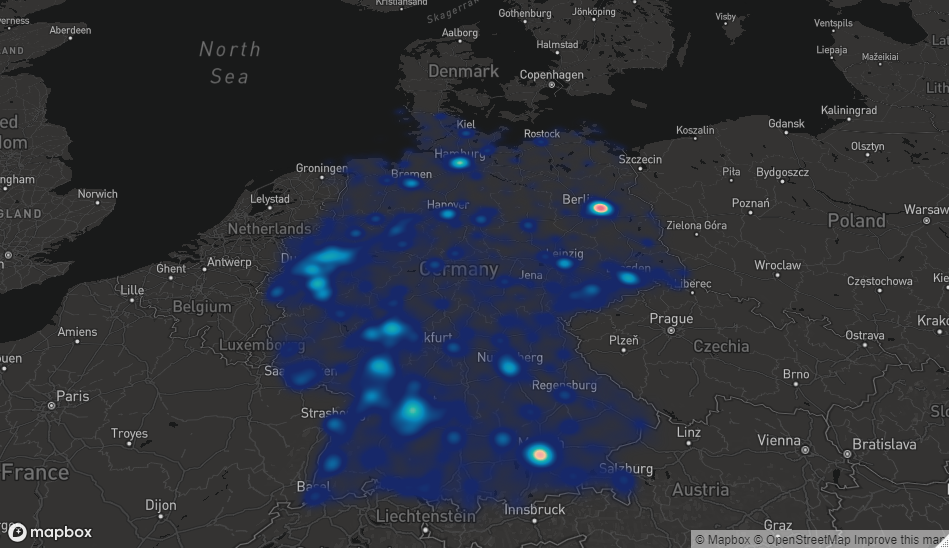
\includegraphics[width = \textwidth]{bakeries_germany_heat.png}
    \caption{A heat map of all bakeries in Germany.}
    \label{fig:map_2}
\end{figure}
Through a choropleth map the number of bakeries in each municipality can be visualized, as seen in Figure~\ref{fig:map_3}.
\begin{figure}[H]
    \centering
    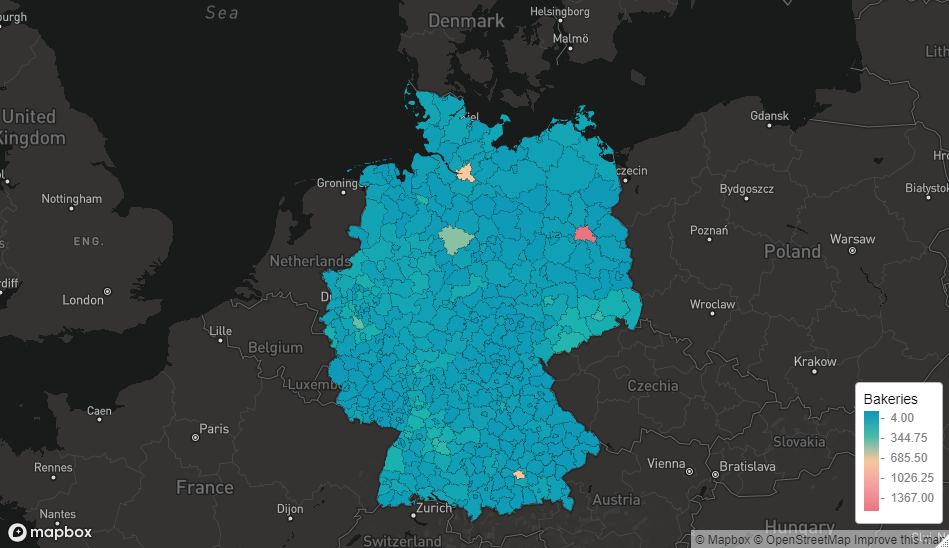
\includegraphics[width = \textwidth]{bakeries_germany_choro.png}
    \caption{A choropleth map of all bakeries in Germany.}
    \label{fig:map_3}
\end{figure}
The app also displays a histogram of the variable selected by the user. Finally, the user has the option to compare a municipality with the rest of the country in terms of indicators of Covid-19 severity. These indicators are the daily number of infections, the total number of infections and the seven-day incidence. This can be used to create charts like the one in Figure~\ref{fig:inc_muc}.
\begin{figure}[H]
    \centering
    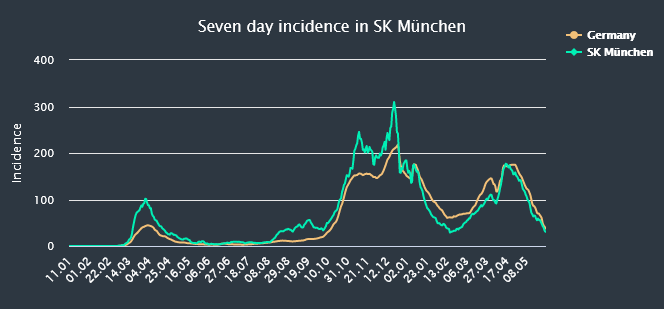
\includegraphics[width = \textwidth]{inc_muc.png}
    \caption{The seven-day incidence in Munich compared to Germany.}
    \label{fig:inc_muc}
\end{figure}
For Europe, the user can view the features used in the fitting of the temporal models. The map can show mobility in different European countries, government measures and general key figures. The user can select a date to see, for example, which measurements were taken at Christmas 2020. Only a choropleth map is available here. Again, the user can view indicators of Covid-19 severity, this time comparing a country with the rest of Europe.
\subsubsection*{The SIR for Norway and Germany}
This is self-explanatory. The user can display the standardized incidence ratio either in Norway or in Germany.
\clearpage
\subsubsection*{Spatial Modelling}
Here the user can fit his own BYM2 model, either for Norway or for Germany. Different variables can be selected to be added to the model, as well as values for $\sigma_0$ and $\alpha$, which are used for the PC prior. After pressing the button to fit the model, which takes a few seconds, the map is updated and the user can now choose to display the relative risk, the posterior mean of the random effects, the exceedance probability or the spatial field. Two tables are also displayed. One containing all relevant performance measures and one containing all significant effects. Each time the user fits a new model, new rows are added to the table. Via the ID column, the user can keep track of his models and see how the performance of a model changes or which effects turn out to be significant in which model.
\subsubsection*{Temporal Modelling}
This is the same as spatial modelling, but this time the user has the option to specify the type of temporal term to use, the country to use for modelling and the test size. The user can choose between five types of temporal terms:
\begin{itemize}
    \item[1.] An iid term
    \item[2.] A random walk of length 1
    \item[3.] A random walk of length 2
    \item[4.] An autoregressive process of order 1
    \item[5.] An Ornstein–Uhlenbeck process
\end{itemize}
33 countries can be selected for modelling and any number can be set for the test size. After the models have been fitted, two graphs are displayed. One for the predicted infection numbers in a country and one for the posterior temporal trend in that country. The graph for the predicted numbers includes a confidence interval for these predictions as well as the actual infection numbers in the country, an example of which can be seen in Figure~\ref{fig:sweden}. \clearpage
\begin{figure}[H]
    \centering
    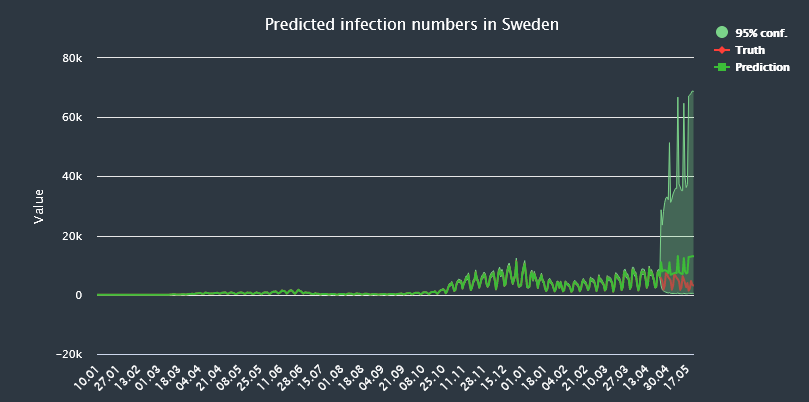
\includegraphics[width = \textwidth]{predicted_sweden.png}
    \caption{Predicted numbers in Sweden using an ar1 model with a test size of 28.}
    \label{fig:sweden}
\end{figure}
The same tables used in the Spatial Modelling tab are also used here and contain the same functionality. \\
The dashboard can be accessed via the following link:
\begin{center}
    \href{https://dashboard.f-hahn.de/}{https://dashboard.f-hahn.de/}
\end{center}